\documentclass[12pt, a4paper]{report}
\usepackage{natbib}
\usepackage{vmargin}
\usepackage{graphicx}
\usepackage{epsfig}
\usepackage{subfigure}
%\usepackage{amscd}
\usepackage{amssymb}
\usepackage{framed}
\usepackage{amsbsy}
\usepackage{amsthm, amsmath}
%\usepackage[dvips]{graphicx}
\bibliographystyle{chicago}
\renewcommand{\baselinestretch}{1.8}

% left top textwidth textheight headheight % headsep footheight footskip
\setmargins{3.0cm}{2.5cm}{15.5 cm}{23.5cm}{0.5cm}{0cm}{1cm}{1cm}

\pagenumbering{arabic}


\begin{document}
	\author{Kevin O'Brien}
	\title{SCRATCH}
	\date{\today}

	
	\tableofcontents \setcounter{tocdepth}{2}
	
	\chapter{The Bland Altman Plot}

	\section{The Bland Altman Plot}
	In 1986 Bland and Altman published a paper in the Lancet proposing
	the difference plot for use for method comparison purposes. It has
	proved highly popular ever since. This is a simple, and widely
	used , plot of the differences of each data pair, and the
	corresponding average value. An important requirement is that the
	two measurement methods use the same scale of measurement.
	\\
	Variations of the Bland Altman plot is the use of ratios, in the
	place of differences.
	\begin{equation}
	D_{i} = X_{i} - Y_{i}   \label{BA01}
	\end{equation}
	Altman and Bland suggest plotting the within subject differences $
	D = X_{1} - X_{2} $ on the ordinate versus the average of $x_{1}$
	and  $x_{2}$ on the abscissa.
	

	
	
	\section{Bland-Altman Plots}
	The issue of whether two measurement methods comparable to the
	extent that they can be used interchangeably with sufficient
	accuracy is encountered frequently in scientific research.
	Historically comparison of two methods of measurement was carried
	out by use of paired sample t-test, correlation coefficients or
	simple linear regression. Statisticians Martin Bland and Douglas
	Altman recognized the inadequacies of these analyses and
	articulated quite thoroughly the basis on which of which they are
	unsuitable for comparing two methods of measurement \citep*{BA83}.
	Furthermore they proposed their simple methodology specifically
	constructed for method comparison studies. They acknowledge the
	opportunity to apply other valid, but complex, methodologies, but
	argue that a simple approach is preferable, especially when the
	results must be `explained to non-statisticians'.
	
	Notwithstanding previous remarks about regression, the first step
	recommended, which the authors argue should be mandatory, is
	construction of a simple scatter plot of the data. The line of
	equality should also be shown, as it is necessary to give the
	correct interpretation of how both methods compare. A scatter plot
	of the Grubbs data is shown in Figure 1.1. Visual inspection confirms the previous conclusion that there is an
	inter-method bias present, i.e. Fotobalk device has a tendency to
	record a lower velocity.
	
	\begin{figure}[h!]
		\begin{center}
			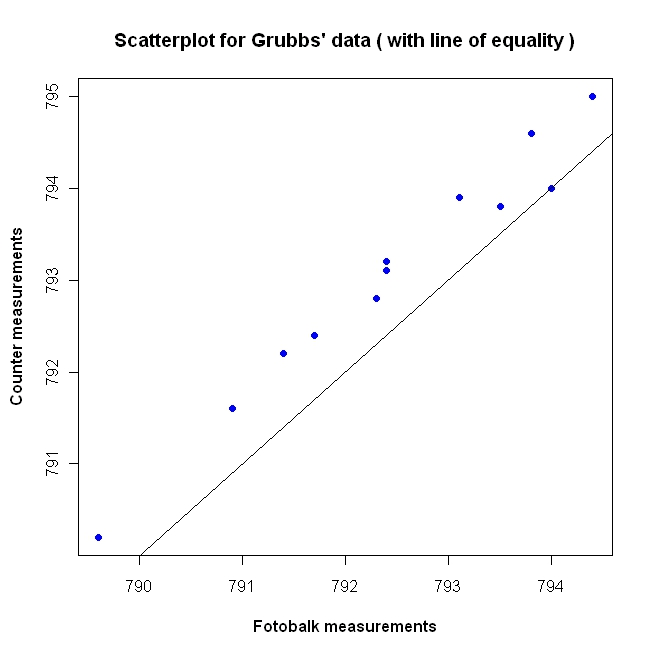
\includegraphics[width=130mm]{images/GrubbsScatter.jpeg}
			\caption{Scatter plot For Fotobalk and Counter Methods.}\label{GrubbsScatter}
		\end{center}
	\end{figure}
	
	In light of shortcomings associated with scatterplots,
	\citet*{BA83} recommend a further analysis of the data. Firstly
	case-wise differences of measurements of two methods $d_{i} =
	y_{1i}-y_{2i} \mbox{ for }i=1,2,..n$ on the same subject should be
	calculated, and then the average of those measurements ($a_{i} =
	(y_{1i} + y_{2i})/2 \mbox{ for }i=1,2,..n$). These differences and
	averages are then plotted. This methodology, now commonly known as
	the `Bland-Altman Plot', has proved very successful.
	\citet*{BA86}, which further develops the methodology, was found
	to be the sixth most cited paper of all time by the
	\citet{BAcite}. \cite{Dewitte} also commented on the rate at which
	prevalence of the Bland-Altman plot has developed in scientific
	literature. The Bland-Altman Plot has since become expected, and
	often obligatory, approach for presenting method comparison
	studies in many scientific journals \citep{hollis}. Furthermore
	\citet{BritHypSoc} recommend its use in papers pertaining to
	method comparison studies for the journal of the British
	Hypertension Society.
	
	The magnitude of the inter-method bias between the two methods is
	simply the average of the differences $\bar{d}$. The variances
	around this bias is estimated by the standard deviation of the
	differences $S(d)$. This inter-method bias is represented with a
	line on the Bland-Altman plot. These estimates are only meaningful
	if there is uniform inter-bias and variability throughout the
	range of measurements, which can be checked by visual inspection
	of the plot. In the case of Grubbs data the inter-method bias is
	$-0.61$ metres per second, and is indicated by the dashed line on
	Figure 1.2. By inspection of the plot, it is also possible to
	compare the precision of each method. Noticeably the differences
	tend to increase as the averages increase.
	
	
	\begin{table}[h!]
		\renewcommand\arraystretch{0.7}%
		\begin{center}
			\begin{tabular}{|c||c|c||c|c|}
				\hline
				Round & Fotobalk  & Counter  & Differences  & Averages  \\
				&  [F] & [C] & [F-C] &  [(F+C)/2] \\
				\hline
				1 & 793.8 & 794.6 & -0.8 & 794.2 \\
				2 & 793.1 & 793.9 & -0.8 & 793.5 \\
				3 & 792.4 & 793.2 & -0.8 & 792.8 \\
				4 & 794.0 & 794.0 & 0.0 & 794.0 \\
				5 & 791.4 & 792.2 & -0.8 & 791.8 \\
				6 & 792.4 & 793.1 & -0.7 & 792.8 \\
				7 & 791.7 & 792.4 & -0.7 & 792.0 \\
				8 & 792.3 & 792.8 & -0.5 & 792.5 \\
				9 & 789.6 & 790.2 & -0.6 & 789.9 \\
				10 & 794.4 & 795.0 & -0.6 & 794.7 \\
				11 & 790.9 & 791.6 & -0.7 & 791.2 \\
				12 & 793.5 & 793.8 & -0.3 & 793.6 \\
				\hline
			\end{tabular}
			\caption{Fotobalk and Counter methods: differences and averages.}
		\end{center}
	\end{table}
	
	\begin{table}[h!]
		\renewcommand\arraystretch{0.7}%
		\begin{center}
			\begin{tabular}{|c||c|c||c|c|}
				\hline
				Round & Fotobalk  & Terma  & Differences  & Averages  \\
				&  [F] & [T] & [F-T] &  [(F+T)/2] \\
				\hline
				1 & 793.80 & 793.20 & 0.60 & 793.50 \\
				2 & 793.10 & 793.30 & -0.20 & 793.20 \\
				3 & 792.40 & 792.60 & -0.20 & 792.50 \\
				4 & 794.00 & 793.80 & 0.20 & 793.90 \\
				5 & 791.40 & 791.60 & -0.20 & 791.50 \\
				6 & 792.40 & 791.60 & 0.80 & 792.00 \\
				7 & 791.70 & 791.60 & 0.10 & 791.65 \\
				8 & 792.30 & 792.40 & -0.10 & 792.35 \\
				9 & 789.60 & 788.50 & 1.10 & 789.05 \\
				10 & 794.40 & 794.70 & -0.30 & 794.55 \\
				11 & 790.90 & 791.30 & -0.40 & 791.10 \\
				12 & 793.50 & 793.50 & 0.00 & 793.50 \\
				
				\hline
			\end{tabular}
			\caption{Fotobalk and Terma methods: differences and averages.}
		\end{center}
	\end{table}
	
	\newpage
	
	
	\subsection{Using Bland-Altman Plots}
	Bland-Altman plots are a powerful graphical methodology for making
	a visual assessment of the data. \citet*{BA83} express the
	motivation for this plot thusly:
	\begin{quote}
		``From this type of plot it is much easier to assess the magnitude
		of disagreement (both error and bias), spot outliers, and see
		whether there is any trend, for example an increase in
		(difference) for high values. This way of plotting the data is a
		very powerful way of displaying the results of a method comparison
		study."
	\end{quote}
	
	The Bland-Altman plot is simply a scatterplot of the case-wise
	averages and differences of two methods of measurement. As the
	objective of the Bland-Altman plot is to advise on the agreement
	of two methods, it is the case-wise differences that are
	particularly. Later it will be shown that case-wise differences
	are the sole component of the next part of the methodology, the
	limits of agreement.
	
	For creating plots, the case wise-averages fulfil several
	functions, such as expressing the range over which the values were
	taken, and assessing whether the assumptions of constant variance
	holds. Case-wise averages also allow the case-wise differences to
	be presented on a two-dimensional plot, with better data
	visualization qualities than a one dimensional plot. \citet{BA86}
	cautions that it would be the difference against either
	measurement value instead of their average , as the difference
	relates to both value.
	
	The Bland-Altman plot for comparing the `Fotobalk' and `Counter'
	methods, which shall henceforth be referred to as the `F vs C'
	comparison,  is depicted in Figure 1.2, using data from Table 1.3.
	The presence and magnitude of the inter-method bias is indicated
	by the dashed line.
	
	\begin{figure}[h!]
		\begin{center}
			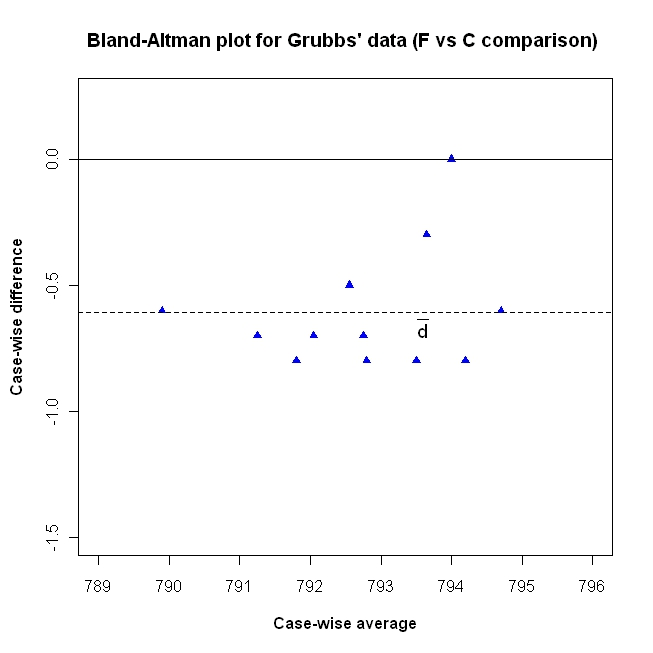
\includegraphics[width=120mm]{images/GrubbsBAplot-noLOA.jpeg}
			\caption{Bland-Altman plot For Fotobalk and Counter methods.}\label{GrubbsBA-noLOA}
		\end{center}
	\end{figure}
	
	
	
	In Figure 1.3 Bland-Altman plots for the `F vs C' and `F vs T'
	comparisons are shown, where `F vs T' refers to the comparison of
	the `Fotobalk' and `Terma' methods. Usage of the Bland-Altman plot
	can be demonstrate in the contrast between these comparisons.
	
	\begin{figure}[h!]
		\begin{center}
			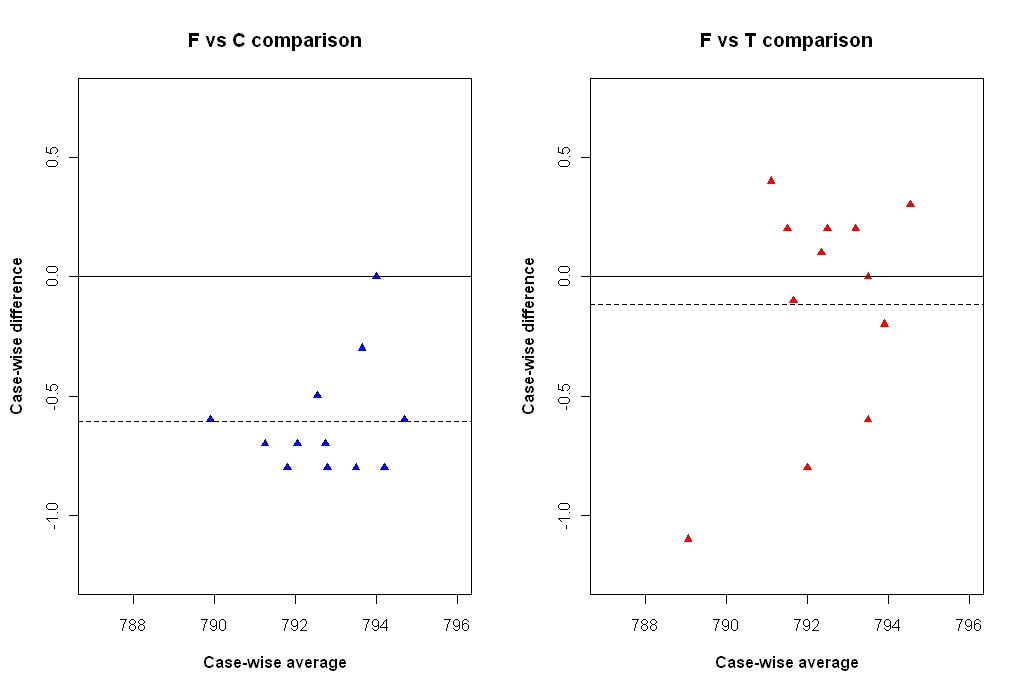
\includegraphics[height=90mm]{images/GrubbsDataTwoBAplots.jpeg}
			\caption{Bland-Altman plots for Grubbs' F vs C and F vs T comparisons.}\label{GrubbsDataTwoBAplots}
		\end{center}
	\end{figure}
	
	By inspection, there exists a larger inter-method bias in the `F
	vs C' comparison than in the `F vs T' comparison. Conversely there
	appears to be less precision in`F vs T' comparison, as indicated
	by the greater dispersion of co-variates.
	
	Figures 1.4, 1.5 and 1.6 are three prototype Bland-Altman plots
	derived from simulated data, each for the purpose of demonstrating
	how the plot would inform an analyst of features that would
	adversely affect use of the recommended methodology.
	
	Figure 1.4 demonstrates how the Bland-Altman plot would indicate
	increasing variance of differences over the measurement range.
	Fitted regression lines, for both the upper and lower half of the
	plot, has been added to indicate the trend. Figure 1.5 is an
	example of cases where the inter-method bias changes over the
	measurement range. This is known as proportional bias. In both
	Figures 1.4 and 1.5, the assumptions necessary for further
	analysis using the limits of agreement are violated.
	
	Application of regression techniques to the Bland-Altman plot, and
	subsequent formal testing for the constant variability of
	differences is informative. The data set may be divided into two
	subsets, containing the observations wherein the difference values
	are less than and greater than the inter-method bias respectively.
	For both of these fits, hypothesis tests for the respective slopes
	can be performed. While both tests can be considered separately,
	multiple comparison procedures, such as the Benjamini-Hochberg
	\citep{BH} test, should be also be used.
	
	\begin{figure}[h!]
		\begin{center}
			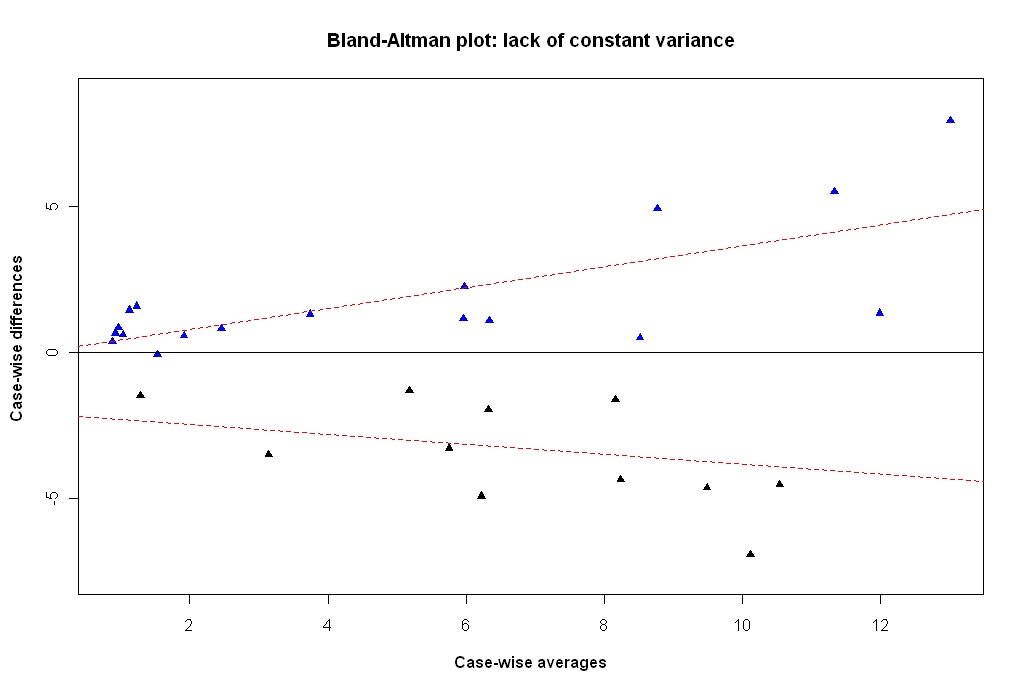
\includegraphics[height=90mm]{images/BAFanEffect.jpeg}
			\caption{Bland-Altman plot demonstrating the increase of variance over the range.}\label{BAFanEffect}
		\end{center}
	\end{figure}
	
	\begin{figure}[h!]
		\begin{center}
			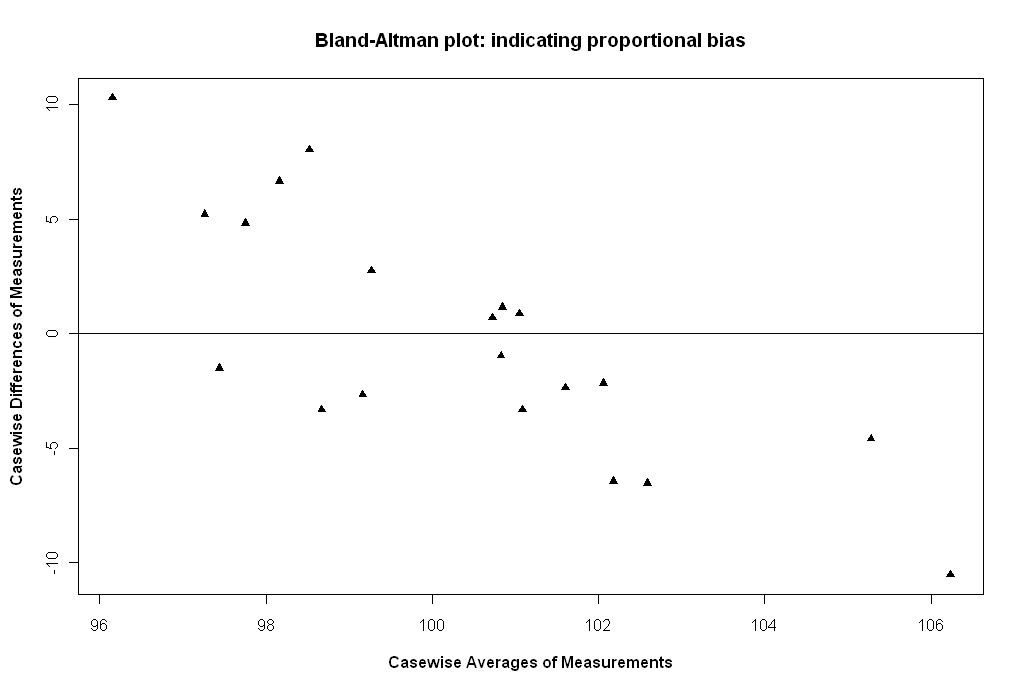
\includegraphics[height=90mm]{images/PropBias.jpeg}
			\caption{Bland-Altman plot indicating the presence of proportional bias.}\label{PropBias}
		\end{center}
	\end{figure}
	
	\begin{figure}[h!]
		\begin{center}
			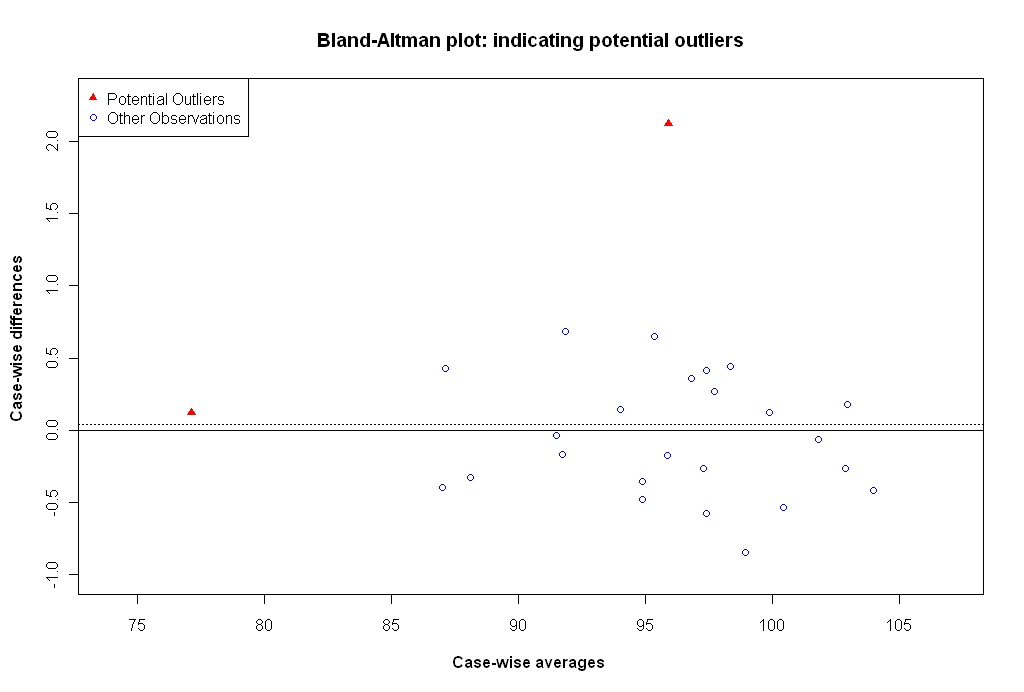
\includegraphics[width=125mm]{images/BAOutliers.jpeg}
			\caption{Bland-Altman plot indicating the presence of potential outliers.}\label{Outliers}
		\end{center}
	\end{figure}
	
	
	% outliers
	
	
	The Bland-Altman plot also can be used to identify outliers. An
	outlier is an observation that is conspicuously different from the
	rest of the data that it arouses suspicion that it occurs due to a
	mechanism, or conditions, different to that of the rest of the
	observations. Classification of outliers can be determined with
	numerous established approaches, such as the Grubb's test, but
	always classification must be informed by the logic of the data's
	formulation. Figure 1.6 is a Bland-Altman plot with two potential
	outliers.
	
	
	\citet*{BA99} do not recommend excluding outliers from analyses,
	but remark that recalculation of the inter-method bias estimate,
	and further calculations based upon that estimate, are useful for
	assessing the influence of outliers. The authors remark that `we
	usually find that this method of analysis is not too sensitive to
	one or two large outlying differences'.
	
	
	%\citet{Grubbs} defined an outlier as a co-variate that appears to
	%deviate markedly from other members of the sample in which it
	%occurs.
	
	In classifying whether a observation from a univariate data set is
	an outlier, Grubbs' outlier test is widely used. In assessing
	whether a co-variate in a Bland-Altman plot is an outlier, this
	test is useful when applied to the difference values treated as a
	univariate data set. For Grubbs' data, this outlier test is
	carried out on the differences, yielding the following results.
	
	The null and alternative hypotheses is the absence and presence of
	at least one outlier respectively. Grubbs' outlier test statistic
	$G$ is the largest absolute deviation from the sample mean divided
	by the standard deviation of the differences. For the `F vs C'
	comparison, $G = 3.6403$. The critical value is calculated using
	Student's $t$ distribution and the sample size,
	\begin{equation}
	U = \frac{n-1}{\sqrt{n}} \sqrt{\frac{t_{\alpha/(2n),n-2}^2}{n - 2
			+ t_{\alpha/(2n),n-2}^2}}.
	\end{equation}
	
	For this test $U = 0.7501$. The conclusion of this test is that
	the fourth observation in the `F vs C' comparison is an outlier,
	with $p-value = 0.002799$.
	
	As a complement to the Bland-Altman plot, \citet{Bartko} proposes
	the use of a bivariate confidence ellipse, constructed for a
	predetermined level.
	
	The minor axis relates to the between subject variability, whereas
	the major axis relates to the error mean square, with the ellipse
	depicting the size of both relative to each
	other.\citet{AltmanEllipse} provides the relevant calculations for
	the ellipse. Bartko states that the ellipse can, inter alia, be
	used to detect the presence of outliers (furthermore
	\citet{Bartko} proposes formal testing procedures, that shall be
	discussed in due course). Inspection of Figure 1.7 shows that the
	fourth observation is outside the bounds of the ellipse,
	concurring with the conclusion that it is an outlier.
	
	
	\begin{figure}[h!]
		% Requires \usepackage{graphicx}
		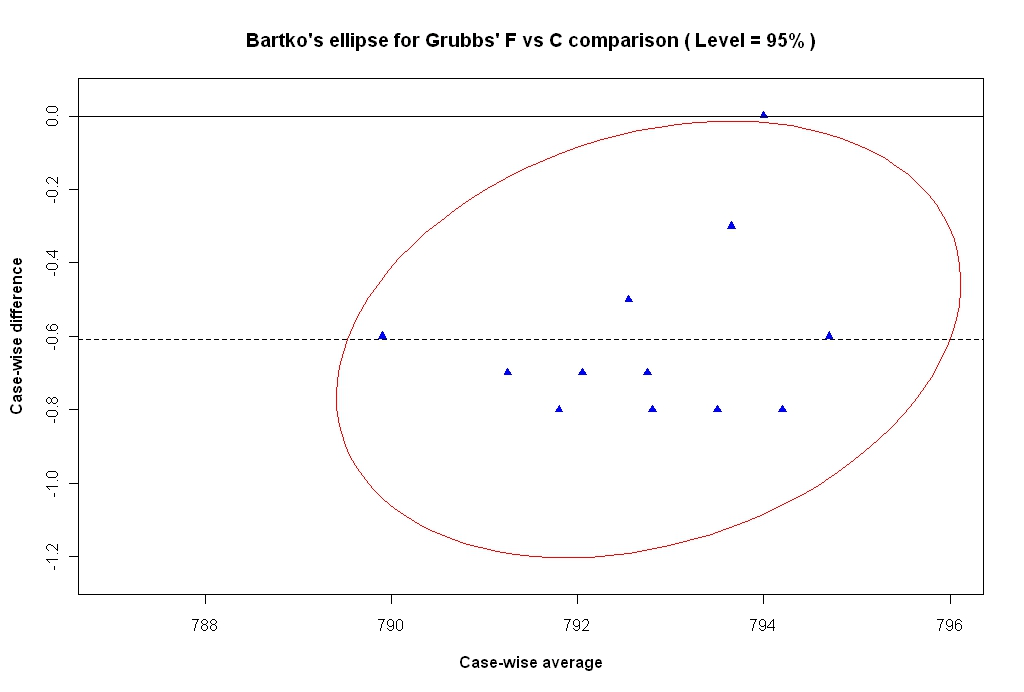
\includegraphics[width=130mm]{images/GrubbsBartko.jpeg}
		\caption{Bartko's Ellipse For Grubbs' Data.}\label{GrubbsBartko}
	\end{figure}
	
	The limitations of using bivariate approaches to outlier detection
	in the Bland-Altman plot can demonstrated using Bartko's ellipse.
	A co-variate is added to the `F vs C' comparison that has a
	difference value equal to the inter-method bias, and an average
	value that markedly deviates from the rest of the average values
	in the comparison, i.e. 786. Table 1.8 depicts a $95\%$ confidence
	ellipse for this enhanced data set. By inspection of the
	confidence interval, a conclusion would be reached that this extra
	co-variate is an outlier, in spite of the fact that this
	observation is consistent with the intended conclusion of the
	Bland-Altman plot.
	
	\begin{figure}[h!]
		% Requires \usepackage{graphicx}
		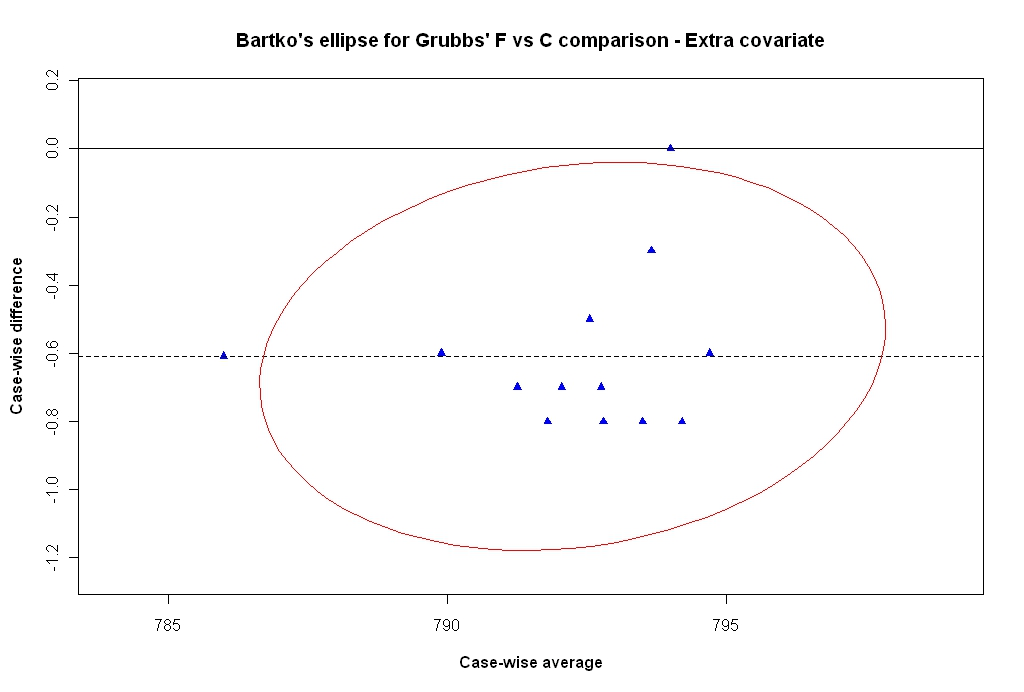
\includegraphics[width=130mm]{images/GrubbsBartko2.jpeg}
		\caption{Bartko's Ellipse For Grubbs' Data, with an extra covariate.}\label{GrubbsBartko2}
	\end{figure}
	
	In the Bland-Altman plot, the horizontal displacement of any
	observation is supported by two independent measurements. Any
	observation should not be considered an outlier on the basis of a
	noticeable horizontal displacement from the main cluster, as in
	the case with the extra co-variate. Conversely, the fourth
	observation, from the original data set, should be considered an
	outlier, as it has a noticeable vertical displacement from the
	rest of the observations.
	
	Bartko's ellipse provides a visual aid to determining the
	relationship between variances. If $\mbox{var}(a_{i})$ is greater
	than $\mbox{var}(d_{i})$, the orientation of the ellipse is
	horizontal. Conversely if $\mbox{var}(a_{i})$ is less than
	$\mbox{var}(d_{i})$, the orientation of the ellipse is vertical.
	\newpage
	
	
	
	%\begin{figure}[h!]
	%\begin{center}
	%  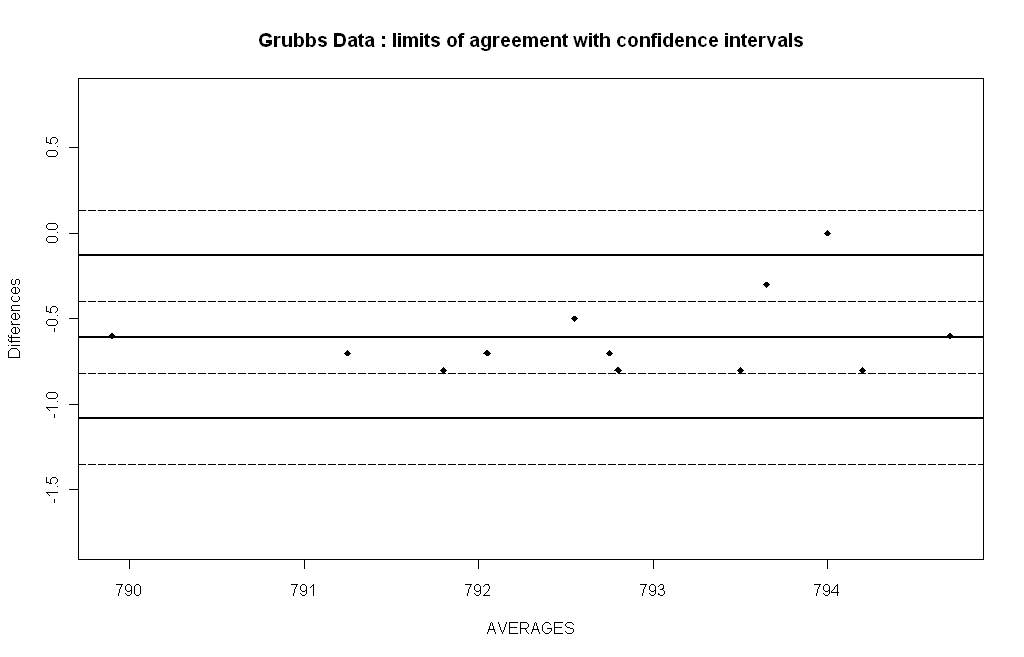
\includegraphics[width=125mm]{images/GrubbsLOAwCIs.jpeg}
	%  \caption{Limits of agreement with confidence intervals}\label{LOAwCIs}
	%\end{center}
	%\end{figure}
	
	\subsection{Using Bland-Altman Plots}
	Bland-Altman plots are a powerful graphical methodology for making
	a visual assessment of the data. \citet*{BA83} express the
	motivation for this plot thusly:
	\begin{quote}
		``From this type of plot it is much easier to assess the magnitude
		of disagreement (both error and bias), spot outliers, and see
		whether there is any trend, for example an increase in
		(difference) for high values. This way of plotting the data is a
		very powerful way of displaying the results of a method comparison
		study."
	\end{quote}
	
	The Bland-Altman plot is simply a scatterplot of the case-wise
	averages and differences of two methods of measurement. As the
	objective of the Bland-Altman plot is to advise on the agreement
	of two methods, it is the case-wise differences that are
	particularly. Later it will be shown that case-wise differences
	are the sole component of the next part of the methodology, the
	limits of agreement.
	
	For creating plots, the case wise-averages fulfil several
	functions, such as expressing the range over which the values were
	taken, and assessing whether the assumptions of constant variance
	holds. Case-wise averages also allow the case-wise differences to
	be presented on a two-dimensional plot, with better data
	visualization qualities than a one dimensional plot. \citet{BA86}
	cautions that it would be the difference against either
	measurement value instead of their average , as the difference
	relates to both value.
	
	The Bland-Altman plot for comparing the `Fotobalk' and `Counter'
	methods, which shall henceforth be referred to as the `F vs C'
	comparison,  is depicted in Figure 1.2, using data from Table 1.3.
	The presence and magnitude of the inter-method bias is indicated
	by the dashed line.
	
	\begin{figure}[h!]
		\begin{center}
			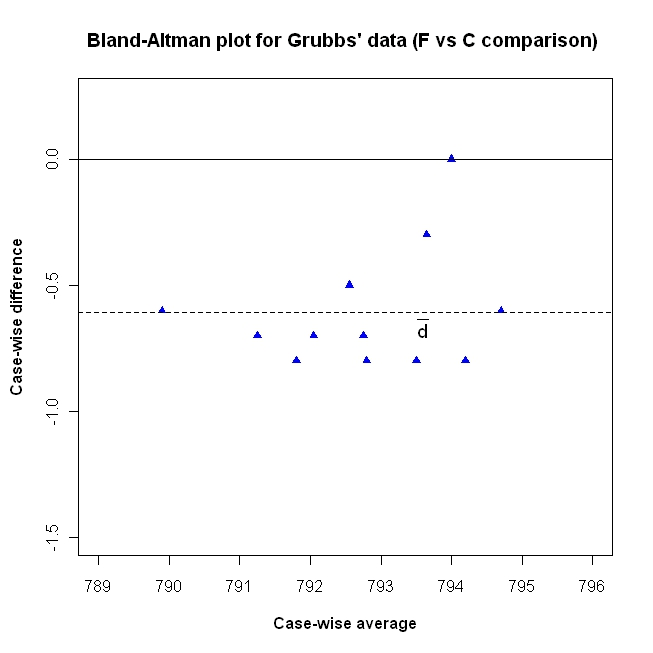
\includegraphics[width=120mm]{images/GrubbsBAplot-noLOA.jpeg}
			\caption{Bland-Altman plot For Fotobalk and Counter methods.}\label{GrubbsBA-noLOA}
		\end{center}
	\end{figure}
	
	
	
	In Figure 1.3 Bland-Altman plots for the `F vs C' and `F vs T'
	comparisons are shown, where `F vs T' refers to the comparison of
	the `Fotobalk' and `Terma' methods. Usage of the Bland-Altman plot
	can be demonstrate in the contrast between these comparisons.
	
	\begin{figure}[h!]
		\begin{center}
			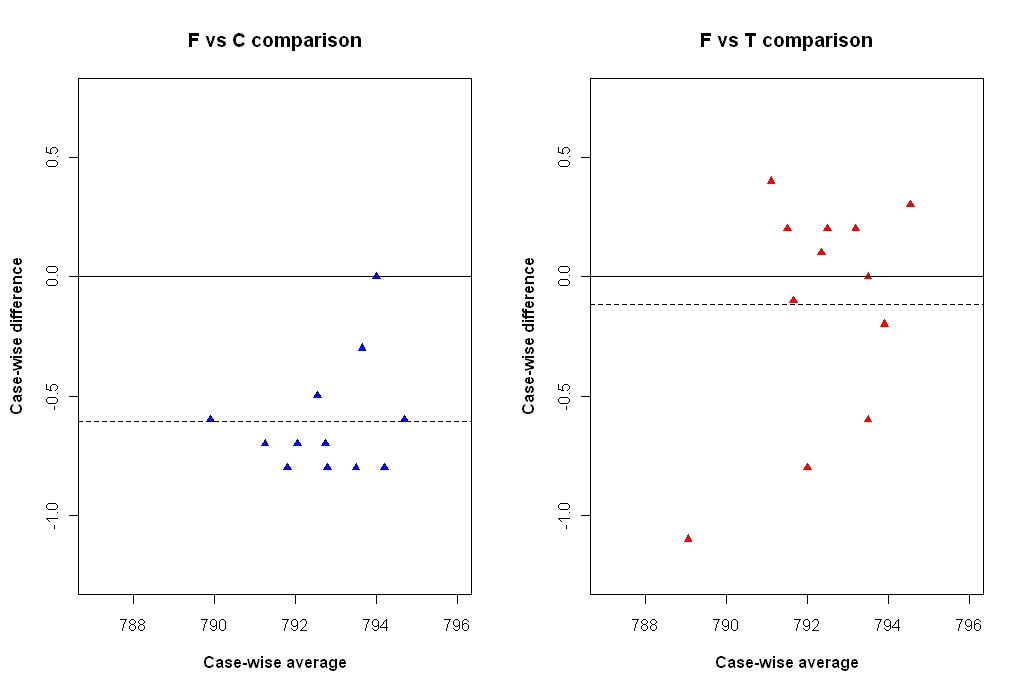
\includegraphics[height=90mm]{images/GrubbsDataTwoBAplots.jpeg}
			\caption{Bland-Altman plots for Grubbs' F vs C and F vs T comparisons.}\label{GrubbsDataTwoBAplots}
		\end{center}
	\end{figure}
	
	By inspection, there exists a larger inter-method bias in the `F
	vs C' comparison than in the `F vs T' comparison. Conversely there
	appears to be less precision in`F vs T' comparison, as indicated
	by the greater dispersion of co-variates.
	
	Figures 1.4, 1.5 and 1.6 are three prototype Bland-Altman plots
	derived from simulated data, each for the purpose of demonstrating
	how the plot would inform an analyst of features that would
	adversely affect use of the recommended methodology.
	
	Figure 1.4 demonstrates how the Bland-Altman plot would indicate
	increasing variance of differences over the measurement range.
	Fitted regression lines, for both the upper and lower half of the
	plot, has been added to indicate the trend. Figure 1.5 is an
	example of cases where the inter-method bias changes over the
	measurement range. This is known as proportional bias. In both
	Figures 1.4 and 1.5, the assumptions necessary for further
	analysis using the limits of agreement are violated.
	
	Application of regression techniques to the Bland-Altman plot, and
	subsequent formal testing for the constant variability of
	differences is informative. The data set may be divided into two
	subsets, containing the observations wherein the difference values
	are less than and greater than the inter-method bias respectively.
	For both of these fits, hypothesis tests for the respective slopes
	can be performed. While both tests can be considered separately,
	multiple comparison procedures, such as the Benjamini-Hochberg
	\citep{BH} test, should be also be used.
	
	\begin{figure}[h!]
		\begin{center}
			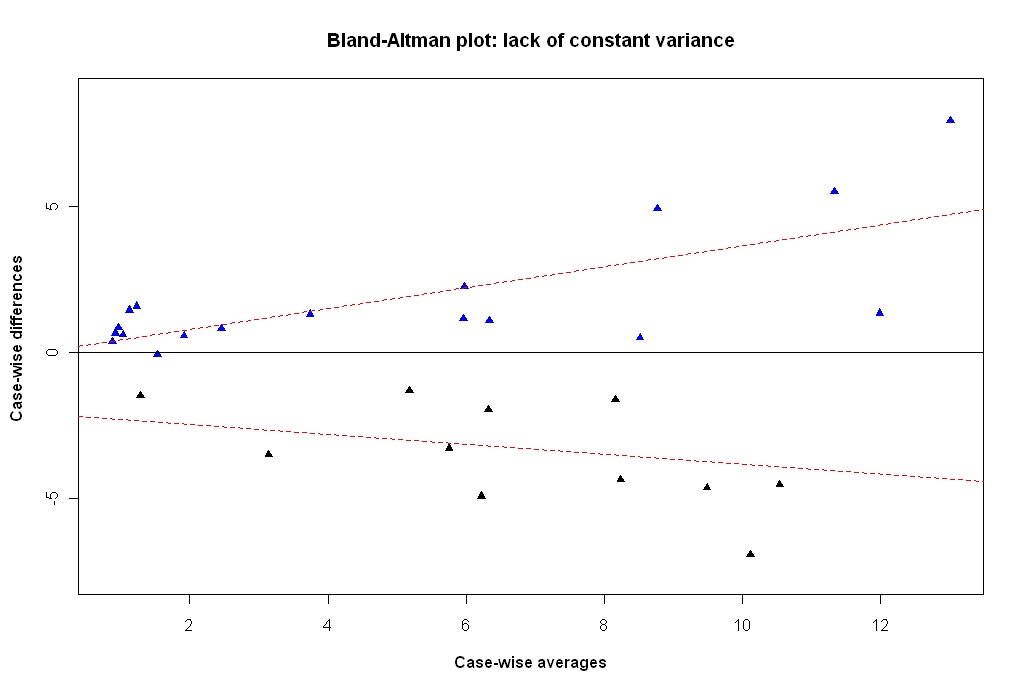
\includegraphics[height=90mm]{images/BAFanEffect.jpeg}
			\caption{Bland-Altman plot demonstrating the increase of variance over the range.}\label{BAFanEffect}
		\end{center}
	\end{figure}
	
	\begin{figure}[h!]
		\begin{center}
			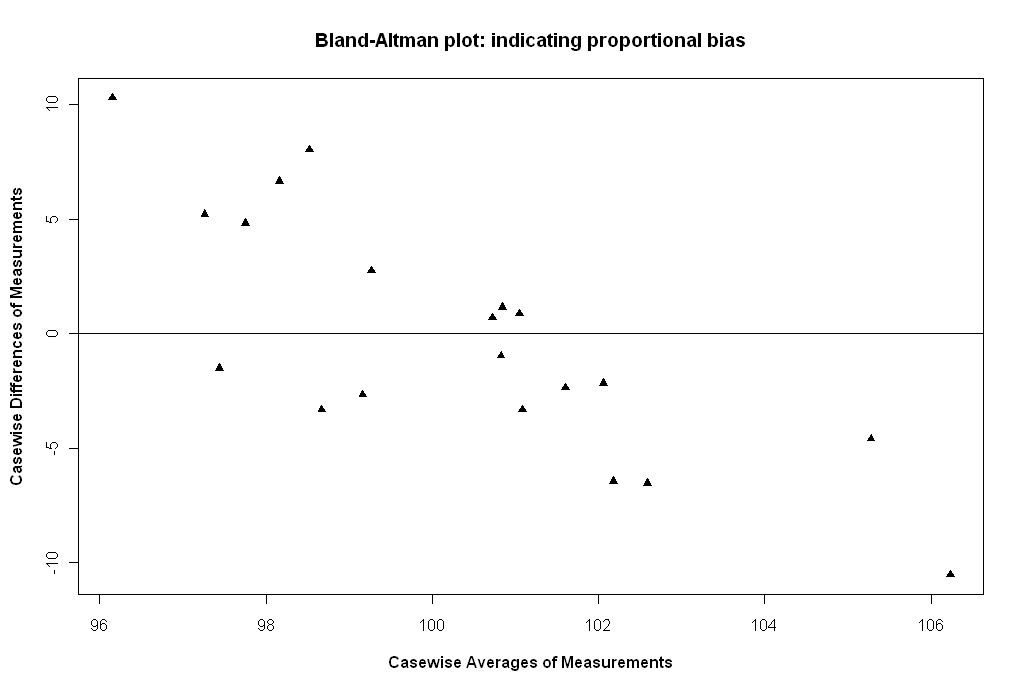
\includegraphics[height=90mm]{images/PropBias.jpeg}
			\caption{Bland-Altman plot indicating the presence of proportional bias.}\label{PropBias}
		\end{center}
	\end{figure}
	
	\begin{figure}[h!]
		\begin{center}
			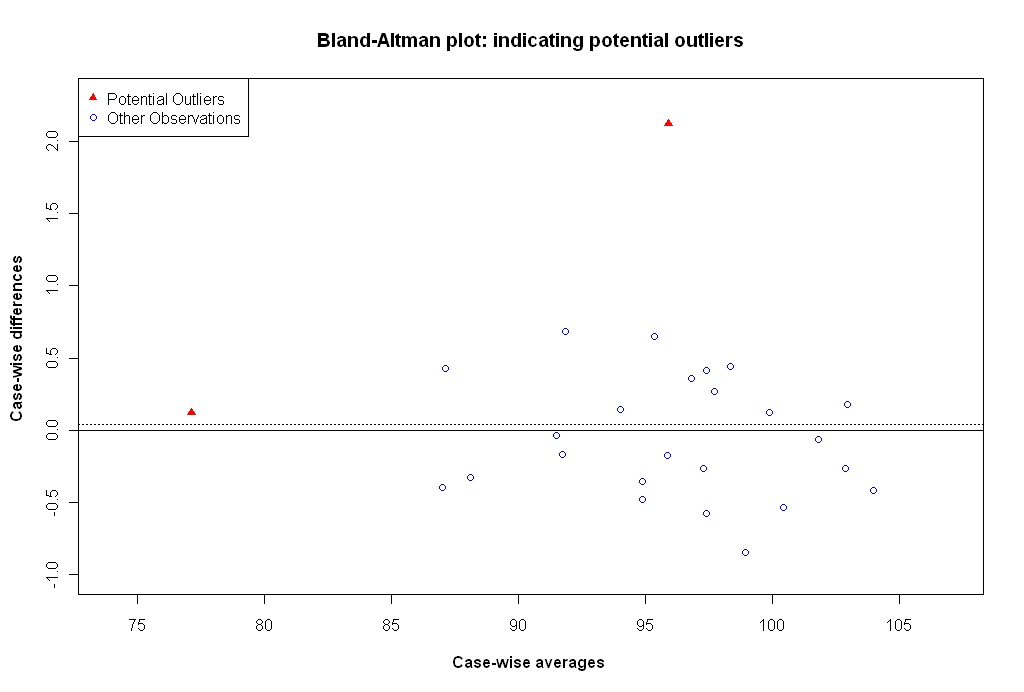
\includegraphics[width=125mm]{images/BAOutliers.jpeg}
			\caption{Bland-Altman plot indicating the presence of potential outliers.}\label{Outliers}
		\end{center}
	\end{figure}
	
	
	% outliers
	
	
	The Bland-Altman plot also can be used to identify outliers. An
	outlier is an observation that is conspicuously different from the
	rest of the data that it arouses suspicion that it occurs due to a
	mechanism, or conditions, different to that of the rest of the
	observations. Classification of outliers can be determined with
	numerous established approaches, such as the Grubb's test, but
	always classification must be informed by the logic of the data's
	formulation. Figure 1.6 is a Bland-Altman plot with two potential
	outliers.
	
	
	\citet*{BA99} do not recommend excluding outliers from analyses,
	but remark that recalculation of the inter-method bias estimate,
	and further calculations based upon that estimate, are useful for
	assessing the influence of outliers. The authors remark that `we
	usually find that this method of analysis is not too sensitive to
	one or two large outlying differences'.
	
	
	%\citet{Grubbs} defined an outlier as a co-variate that appears to
	%deviate markedly from other members of the sample in which it
	%occurs.
	
	In classifying whether a observation from a univariate data set is
	an outlier, Grubbs' outlier test is widely used. In assessing
	whether a co-variate in a Bland-Altman plot is an outlier, this
	test is useful when applied to the difference values treated as a
	univariate data set. For Grubbs' data, this outlier test is
	carried out on the differences, yielding the following results.
	
	The null and alternative hypotheses is the absence and presence of
	at least one outlier respectively. Grubbs' outlier test statistic
	$G$ is the largest absolute deviation from the sample mean divided
	by the standard deviation of the differences. For the `F vs C'
	comparison, $G = 3.6403$. The critical value is calculated using
	Student's $t$ distribution and the sample size,
	\begin{equation}
	U = \frac{n-1}{\sqrt{n}} \sqrt{\frac{t_{\alpha/(2n),n-2}^2}{n - 2
			+ t_{\alpha/(2n),n-2}^2}}.
	\end{equation}
	
	For this test $U = 0.7501$. The conclusion of this test is that
	the fourth observation in the `F vs C' comparison is an outlier,
	with $p-value = 0.002799$.
	
	As a complement to the Bland-Altman plot, \citet{Bartko} proposes
	the use of a bivariate confidence ellipse, constructed for a
	predetermined level.
	
	The minor axis relates to the between subject variability, whereas the major axis relates to the error mean square, with the ellipse
	depicting the size of both relative to each	other.\citet{AltmanEllipse} provides the relevant calculations for
	the ellipse. Bartko states that the ellipse can, inter alia, be
	used to detect the presence of outliers (furthermore \citet{Bartko} proposes formal testing procedures, that shall be
	discussed in due course). Inspection of Figure 1.7 shows that the
	fourth observation is outside the bounds of the ellipse, concurring with the conclusion that it is an outlier.
	
	
	\begin{figure}[h!]
		% Requires \usepackage{graphicx}
		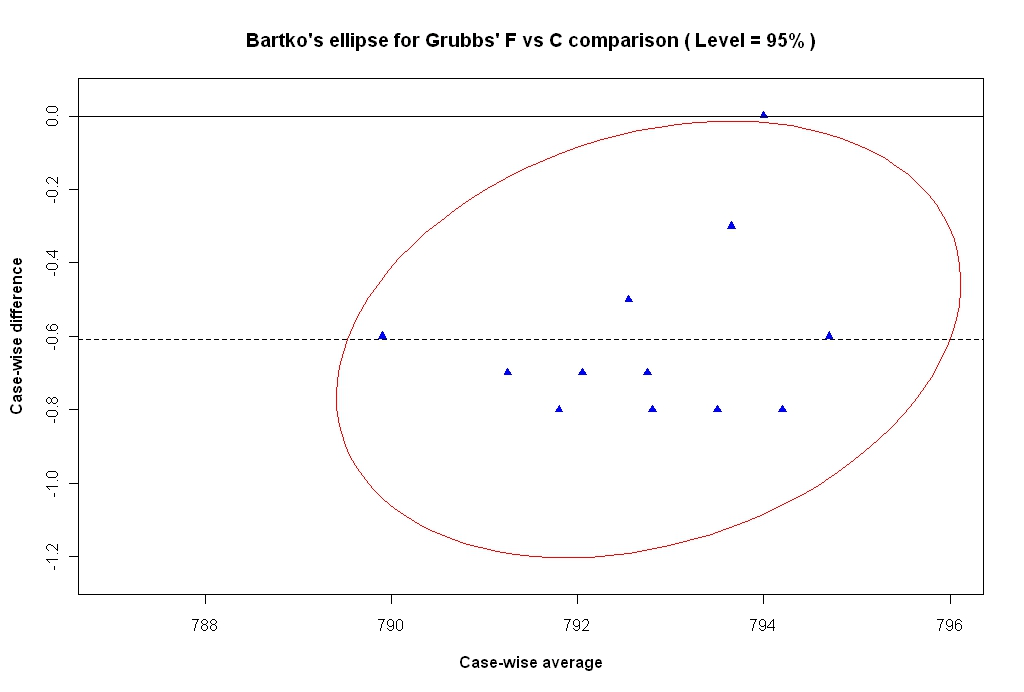
\includegraphics[width=130mm]{images/GrubbsBartko.jpeg}
		\caption{Bartko's Ellipse For Grubbs' Data.}\label{GrubbsBartko}
	\end{figure}
	
	The limitations of using bivariate approaches to outlier detection
	in the Bland-Altman plot can demonstrated using Bartko's ellipse.
	A co-variate is added to the `F vs C' comparison that has a	difference value equal to the inter-method bias, and an average	value that markedly deviates from the rest of the average values in the comparison, i.e. 786. Table 1.8 depicts a $95\%$ confidence
	ellipse for this enhanced data set. By inspection of the confidence interval, a conclusion would be reached that this extra
	co-variate is an outlier, in spite of the fact that this observation is consistent with the intended conclusion of the
	Bland-Altman plot.
	
	\begin{figure}[h!]
		% Requires \usepackage{graphicx}
		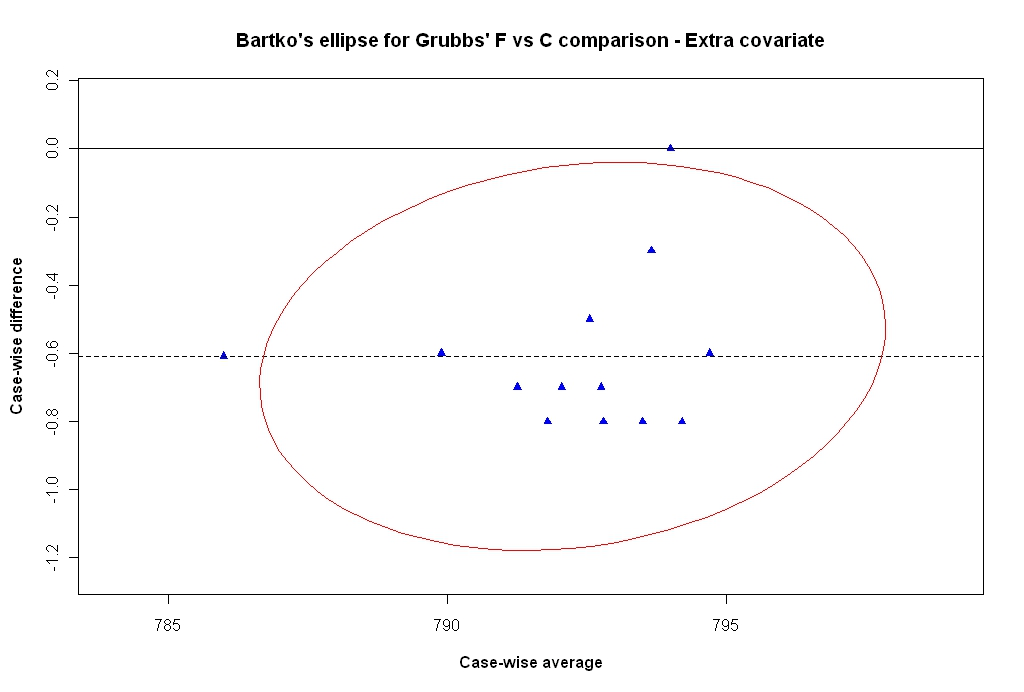
\includegraphics[width=130mm]{images/GrubbsBartko2.jpeg}
		\caption{Bartko's Ellipse For Grubbs' Data, with an extra covariate.}\label{GrubbsBartko2}
	\end{figure}
	
	In the Bland-Altman plot, the horizontal displacement of any observation is supported by two independent measurements. Any
	observation should not be considered an outlier on the basis of a
	noticeable horizontal displacement from the main cluster, as in
	the case with the extra co-variate. Conversely, the fourth observation, from the original data set, should be considered an
	outlier, as it has a noticeable vertical displacement from the rest of the observations.
	
	Bartko's ellipse provides a visual aid to determining the relationship between variances. If $\mbox{var}(a_{i})$ is greater
	than $\mbox{var}(d_{i})$, the orientation of the ellipse is	horizontal. Conversely if $\mbox{var}(a_{i})$ is less than
	$\mbox{var}(d_{i})$, the orientation of the ellipse is vertical.
	\newpage
	
	
	
	%\begin{figure}[h!]
	%\begin{center}
	%  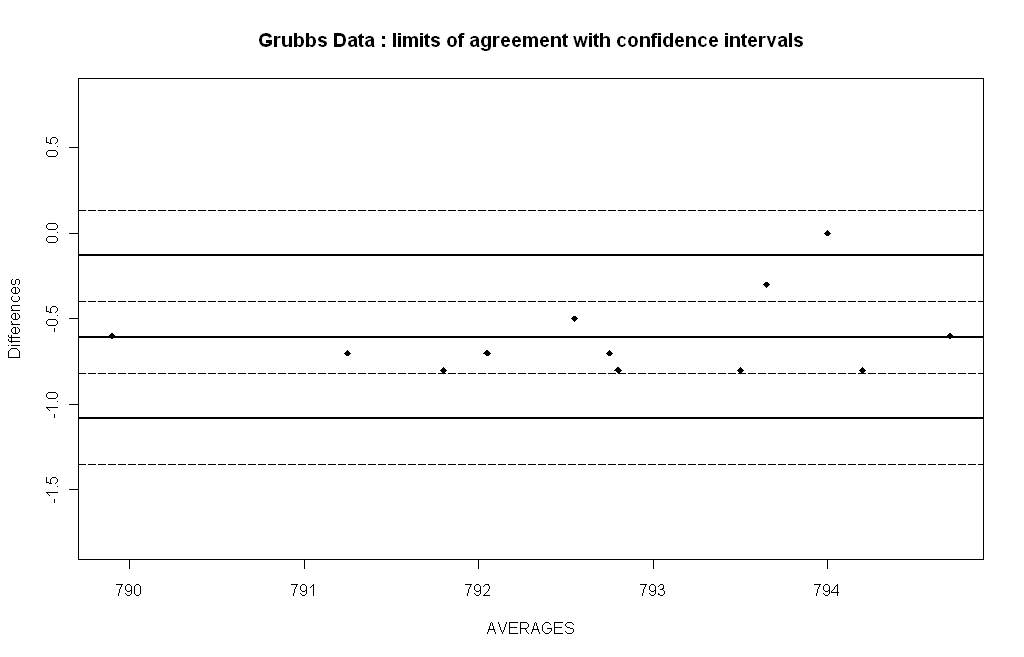
\includegraphics[width=125mm]{images/GrubbsLOAwCIs.jpeg}
	%  \caption{Limits of agreement with confidence intervals}\label{LOAwCIs}
	%\end{center}
	%\end{figure}
	
	%================================================================ %
	% USED
	\subsection{Variations of the Bland-Altman Plot} Referring to the
	assumption that bias and variability are constant across the range
	of measurements, \citet{BA99} address the case where there is an
	increase in variability as the magnitude increases. They remark
	that it is possible to ignore the issue altogether, but the limits
	of agreement would wider apart than necessary when just lower
	magnitude measurements are considered. Conversely the limits would
	be too narrow should only higher magnitude measurements be used.
	To address the issue, they propose the logarithmic transformation
	of the data. The plot is then formulated as the difference of
	paired log values against their mean. Bland and Altman acknowledge
	that this is not easy to interpret, and may not be suitable in
	all cases.
	
	\citet{BA99} offers two variations of the Bland-Altman plot that
	are intended to overcome potential problems that the conventional
	plot would inappropriate for. The first variation is a plot of
	casewise differences as percentage of averages, and is appropriate
	when there is an increase in variability of the differences as the
	magnitude increases. The second variation is a plot of casewise
	ratios as percentage of averages. This will remove the need for
	log transformation. This approach is useful when there is an
	increase in variability of the differences as the magnitude of the
	measurement increases. \citet{Eksborg} proposed such a ratio plot,
	independently of Bland and Altman. \citet{Dewitte} commented on
	the reception of this article by saying `Strange to say,this
	report has been overlooked'.
	
	
	
	
	\subsection{Variations of the Bland-Altman Plot} Referring to the
	assumption that bias and variability are constant across the range
	of measurements, \citet{BA99} address the case where there is an
	increase in variability as the magnitude increases. They remark
	that it is possible to ignore the issue altogether, but the limits
	of agreement would wider apart than necessary when just lower
	magnitude measurements are considered. Conversely the limits would
	be too narrow should only higher magnitude measurements be used.
	To address the issue, they propose the logarithmic transformation
	of the data. The plot is then formulated as the difference of
	paired log values against their mean. Bland and Altman acknowledge
	that this is not easy to interpret, and may not be suitable in
	all cases.
	
	\citet{BA99} offers two variations of the Bland-Altman plot that
	are intended to overcome potential problems that the conventional
	plot would inappropriate for. The first variation is a plot of
	casewise differences as percentage of averages, and is appropriate
	when there is an increase in variability of the differences as the
	magnitude increases. The second variation is a plot of casewise
	ratios as percentage of averages. This will remove the need for
	log transformation. This approach is useful when there is an
	increase in variability of the differences as the magnitude of the
	measurement increases. \citet{Eksborg} proposed such a ratio plot,
	independently of Bland and Altman. \citet{Dewitte} commented on
	the reception of this article by saying `Strange to say,this
	report has been overlooked'.
	%USED
	%=============================================== %
	
	
	
	
	

	\subsection{Regression-based Limits of Agreement} Assuming that
	there will be no curvature in the scatter-plot, the methodology
	regresses the difference of methods ($d$) on the average of those
	methods ($a$) with a simple intercept slope model; $\hat{d} =
	b_{0}+ b_{1}a.$ Should the slope $b_{1}$ be found to be
	negligible, $\hat{d}$ takes the value $\bar{d}$.
	
	The next step to take in calculating the limits is also a
	regression, this time of the residuals as a function of the scale
	of the measurements, expressed by the averages $a_{i}$;
	$ \hat{R} = c_{0}+ c_{1}a_{i}$
	
	With reference to absolute values following a half-normal
	distribution with mean $\sigma\sqrt{\frac{2}{\pi}}$, \citet{BA99} formulate the regression based limits of agreement as
	follows
	\begin{equation}
	\hat{d} \pm 1.96\sqrt{\frac{\pi}{2}}\hat{R} = \hat{d} \pm 2.46\hat{R}
	\end{equation}
	
	\subsection{Regression-based Limits of Agreement} Assuming that
	there will be no curvature in the scatter-plot, the methodology
	regresses the difference of methods ($d$) on the average of those
	methods ($a$) with a simple intercept slope model; $\hat{d} =
	b_{0}+ b_{1}a.$ Should the slope $b_{1}$ be found to be
	negligible, $\hat{d}$ takes the value $\bar{d}$.
	
	The next step to take in calculating the limits is also a
	regression, this time of the residuals as a function of the scale
	of the measurements, expressed by the averages $a_{i}$;
	$ \hat{R} = c_{0}+ c_{1}a_{i}$
	
	With reference to absolute values following a half-normal
	distribution with mean $\sigma\sqrt{\frac{2}{\pi}}$, \citet{BA99} formulate the regression based limits of agreement as
	follows
	\begin{equation}
	\hat{d} \pm 1.96\sqrt{\frac{\pi}{2}}\hat{R} = \hat{d} \pm 2.46\hat{R}
	\end{equation}

	\subsection{Replicate Measurements}
	
	Thus far, the formulation for comparison of two measurement
	methods is one where one measurement by each method is taken on
	each subject. Should there be two or more measurements by each
	methods, these measurement are known as `replicate measurements'.
	\citet{BXC2008} recommends the use of replicate measurements, but
	acknowledges that  additional computational complexity.
	
	\citet*{BA86} address this problem by offering two different approaches. The premise of the first approach is that replicate
	measurements can be treated as independent measurements. The
	second approach is based upon using the mean of the each group of
	replicates as a representative value of that group. Using either
	of these approaches will allow an analyst to estimate the inter
	method bias.
	
	%\subsubsection{Mean of Replicates Limits of Agreement}
	
	However, because of the removal of the effects of the replicate	measurements error, this would cause the estimation of the
	standard deviation of the differences to be unduly small.
	\citet*{BA86} propose a correction for this.
	
	\citet{BXC2008} takes issue with the limits of agreement based on
	mean values, in that they can only be interpreted as prediction
	limits for difference between means of repeated measurements by
	both methods, as opposed to the difference of all measurements.
	Incorrect conclusions would be caused by such a misinterpretation.
	\citet{BXC2008} demonstrates how the limits of agreement
	calculated using the mean of replicates are `much too narrow as
	prediction limits for differences between future single
	measurements'. This paper also comments that, while treating the
	replicate measurements as independent will cause a downward bias
	on the limits of agreement calculation, this method is preferable
	to the `mean of replicates' approach.
	
	The approach proposed by \citet{BA83} is a formal test on the Pearson correlation coefficient of case-wise differences and means
	($\rho_{ad}$). According to the authors, this test is equivalent
	to the `Pitman Morgan Test'. For the Grubbs data, the correlation
	coefficient estimate ($r_{ad}$) is 0.2625, with a 95\% confidence
	interval of (-0.366, 0.726) estimated by Fishers `r to z'
	transformation \citep*{Cohen}. The null hypothesis ($\rho_{ad}$
	=0)would fail to be rejected. Consequently the null hypothesis of
	equal variances of each method would also fail to be rejected.
	There has no been no further mention of this particular test in
	\citet{BA86}, although \citet{BA99} refers to Spearman's rank
	correlation coefficient. \citet{BA99} comments `we do not see a
	place for methods of analysis based on hypothesis testing'.
	\citet{BA99} also states that consider structural equation models
	to be inappropriate.
	
	\citet{DunnSEME} highlights an important issue regarding using
	models such as these, the identifiability problem. This comes as a
	result of there being too many parameters to be estimated.
	Therefore assumptions about some parameters, or estimators used,
	must be made so that others can be estimated. For example $\alpha$
	may take the value of the inter-method bias estimate from
	Bland-Altman methodology. Another assumption is that the precision
	ratio $\lambda=\frac{\sigma^{2}_{\epsilon}}{\sigma^{2}_{\delta}}$
	may be known.
	
	
	\citet{DunnSEME} considers methodologies based on two methods with single measurements on each subject as inadequate for a serious study
	on the measurement characteristics of the methods. This is because there would not be enough data to allow for a meaningful analysis.
	There is, however, a contrary argument that is very difficult to get replicate
	observations when the measurement method requires invasive medical procedure.
	
	\citet{DunnSEME} recommends the following approach for analyzing
	method comparison data. Firstly he recommends conventional
	Bland-Altman methodology; plotting the scatterplot and the
	Bland-Altman plot, complemented by estimate for the limits of
	agreement and the correlation coefficient between the difference
	and the mean. Additionally boxplots may be useful in considering
	the marginal distributions of the observations. The second step is
	the calculations of summary statistics; the means and variances of
	each set of measurements, and the covariances.
	%Should covariance values be greater than the either of the two variances,
	
	When both methods measure in the same scale (i.e. $\beta = 1$),
	\citet{DunnSEME} recommends the use of Grubbs estimators to
	estimate error variances, and to test for their equality. A test
	of whether the intercept $\alpha$ may be also be appropriate.
	
	
	
	%This application of the
	%Grubbs method presumes the existence of this condition, and necessitates
	%replication of observations by means external to and independent of the first
	%means. The Grubbs estimators method is based on the laws of propagation of
	%error. By making three independent simultaneous measurements on the same
	%physical material, it is possible by appropriate mathematical manipulation of
	%the sums and differences of the associated variances to obtain a valid
	%estimate of the precision of the primary means. Application of the Grubbs
	%estimators procedure to estimation of the precision of an apparatus uses
	%the results of a physical test conducted in such a way as to obtain a series
	%of sets of three independent observations.
	
	
	
	%%%%%%%%%%%%%%%%%%%%%%%%%%%%%%%%%%%%%%%%%%%%%%%%%%%%%%%%%%%%%%%%%%%%%%%%%%%%%%%%%%%%%%%%%%%%%%%%%%%%%%%%
	
	
	\newpage
	% latex table generated in R 2.6.0 by xtable 1.5-5 package
	% Thu Aug 27 16:31:52 2009
	\begin{table}[tbh]
		\begin{center}
			
			\begin{tabular}{|c|c|c|c|c|}
				\hline
				Round & Fotobalk [F] & Counter [C] & Differences [F-C] & Averages [(F+C)/2] \\
				\hline
				1 & 793.80 & 794.60 & -0.80 & 794.20 \\
				2 & 793.10 & 793.90 & -0.80 & 793.50 \\
				3 & 792.40 & 793.20 & -0.80 & 792.80 \\
				4 & 794.00 & 794.00 & 0.00 & 794.00 \\
				5 & 791.40 & 792.20 & -0.80 & 791.80 \\
				6 & 792.40 & 793.10 & -0.70 & 792.80 \\
				7 & 791.70 & 792.40 & -0.70 & 792.00 \\
				8 & 792.30 & 792.80 & -0.50 & 792.50 \\
				9 & 789.60 & 790.20 & -0.60 & 789.90 \\
				10 & 794.40 & 795.00 & -0.60 & 794.70 \\
				11 & 790.90 & 791.60 & -0.70 & 791.20 \\
				12 & 793.50 & 793.80 & -0.30 & 793.60 \\
				\hline
			\end{tabular}
			\caption{Fotobalk and Counter Methods: Differences and Averages}
		\end{center}
	\end{table}
	
	
	
	


	\subsection{Replicate Measurements}
	
	Thus far, the formulation for comparison of two measurement
	methods is one where one measurement by each method is taken on
	each subject. Should there be two or more measurements by each
	methods, these measurement are known as `replicate measurements'.
	\citet{BXC2008} recommends the use of replicate measurements, but
	acknowledges that  additional computational complexity.
	
	\citet*{BA86} address this problem by offering two different
	approaches. The premise of the first approach is that replicate
	measurements can be treated as independent measurements. The
	second approach is based upon using the mean of the each group of
	replicates as a representative value of that group. Using either
	of these approaches will allow an analyst to estimate the inter
	method bias.
	
	%\subsubsection{Mean of Replicates Limits of Agreement}
	
	However, because of the removal of the effects of the replicate
	measurements error, this would cause the estimation of the
	standard deviation of the differences to be unduly small.
	\citet*{BA86} propose a correction for this.
	
	\citet{BXC2008} takes issue with the limits of agreement based on
	mean values, in that they can only be interpreted as prediction
	limits for difference between means of repeated measurements by
	both methods, as opposed to the difference of all measurements.
	Incorrect conclusions would be caused by such a misinterpretation.
	\citet{BXC2008} demonstrates how the limits of agreement
	calculated using the mean of replicates are `much too narrow as
	prediction limits for differences between future single
	measurements'. This paper also comments that, while treating the
	replicate measurements as independent will cause a downward bias
	on the limits of agreement calculation, this method is preferable
	to the `mean of replicates' approach.
	
	The approach proposed by \citet{BA83} is a formal test on the
	Pearson correlation coefficient of case-wise differences and means
	($\rho_{ad}$). According to the authors, this test is equivalent
	to the `Pitman Morgan Test'. For the Grubbs data, the correlation
	coefficient estimate ($r_{ad}$) is 0.2625, with a 95\% confidence
	interval of (-0.366, 0.726) estimated by Fishers `r to z'
	transformation \citep*{Cohen}. The null hypothesis ($\rho_{ad}$
	=0)would fail to be rejected. Consequently the null hypothesis of
	equal variances of each method would also fail to be rejected.
	There has no been no further mention of this particular test in
	\citet{BA86}, although \citet{BA99} refers to Spearman's rank
	correlation coefficient. \citet{BA99} comments `we do not see a
	place for methods of analysis based on hypothesis testing'.
	\citet{BA99} also states that consider structural equation models
	to be inappropriate.
	
	\citet{DunnSEME} highlights an important issue regarding using
	models such as these, the identifiability problem. This comes as a
	result of there being too many parameters to be estimated.
	Therefore assumptions about some parameters, or estimators used,
	must be made so that others can be estimated. For example $\alpha$
	may take the value of the inter-method bias estimate from
	Bland-Altman methodology. Another assumption is that the precision
	ratio $\lambda=\frac{\sigma^{2}_{\epsilon}}{\sigma^{2}_{\delta}}$
	may be known.
	
	
	\citet{DunnSEME} considers methodologies based on two methods with single measurements on each subject as inadequate for a serious study
	on the measurement characteristics of the methods. This is because there would not be enough data to allow for a meaningful analysis.
	There is, however, a contrary argument that is very difficult to get replicate
	observations when the measurement method requires invasive medical procedure.
	
	\citet{DunnSEME} recommends the following approach for analyzing
	method comparison data. Firstly he recommends conventional
	Bland-Altman methodology; plotting the scatterplot and the
	Bland-Altman plot, complemented by estimate for the limits of
	agreement and the correlation coefficient between the difference
	and the mean. Additionally boxplots may be useful in considering
	the marginal distributions of the observations. The second step is
	the calculations of summary statistics; the means and variances of
	each set of measurements, and the covariances.
	%Should covariance values be greater than the either of the two variances,
	
	When both methods measure in the same scale (i.e. $\beta = 1$),
	\citet{DunnSEME} recommends the use of Grubbs estimators to
	estimate error variances, and to test for their equality. A test
	of whether the intercept $\alpha$ may be also be appropriate.
	
	
	
	%This application of the
	%Grubbs method presumes the existence of this condition, and necessitates
	%replication of observations by means external to and independent of the first
	%means. The Grubbs estimators method is based on the laws of propagation of
	%error. By making three independent simultaneous measurements on the same
	%physical material, it is possible by appropriate mathematical manipulation of
	%the sums and differences of the associated variances to obtain a valid
	%estimate of the precision of the primary means. Application of the Grubbs
	%estimators procedure to estimation of the precision of an apparatus uses
	%the results of a physical test conducted in such a way as to obtain a series
	%of sets of three independent observations.
	
	

	
	
	
	
	
	
	

\subsection{Repeated Measurements }
In cases where there are repeated measurements by each of the two
methods on the same subjects , Bland Altman suggest calculating
the mean for each method on each subject and use these pairs of
means to compare the two methods.
\\
The estimate of bias will be unaffected using this approach, but
the estimate of the standard deviation of the differences will be
too small, because of the reduction of the effect of repeated
measurement error. Bland Altman propose a correction for this.
\\
Carstensen attends to this issue also, adding that another
approach would be to treat each repeated measurement separately.







	\section{Bland Altman Plots}
	The issue of whether two measurement methods are comparable to the
	extent that they can be used interchangeably with sufficient
	accuracy is encountered frequently in scientific research.
	Historically comparison of two methods of measurement was carried
	out by use of matched pairs correlation coefficients or simple
	linear regression. Bland and Altman recognized the inadequacies of
	these analyses and articulated quite thoroughly the basis on which
	of which they are unsuitable for comparing two methods of
	measurement \citep*{BA83}.
	
	As an alternative they proposed a simple statistical methodology
	specifically appropriate for method comparison studies. They
	acknowledge that there are other valid methodologies, but argue
	that a simple approach is preferable to complex approaches,
	\emph{"especially when the results must be explained to
		non-statisticians"} \citep*{BA83}.
	
	The first step recommended which the authors argue should be
	mandatory is construction of a simple scatter plot of the data.
	The line of equality ($X=Y$) should also be shown, as it is
	necessary to give the correct interpretation of how both methods
	compare. A scatter plot of the Grubbs data is shown in figure 2.1.
	A visual inspection thereof confirms the previous conclusion that
	there is an inter method bias present, i.e. Fotobalk device has a
	tendency to record a lower velocity.
	
	
	
	In light of shortcomings associated with scatterplots,
	\citet*{BA83} recommend a further analysis of the data. Firstly
	differences of measurements of two methods on the same subject
	should  be calculated, and then the average of those measurements
	(Table 1.1). The averages of the two measurements is considered by
	Bland and Altman to the best estimate for the unknown true value.
	Importantly both methods must measure with the same units. These
	results are then plotted, with differences on the ordinate and
	averages on the abscissa (figure 1.2). \citet*{BA83}express the
	motivation for this plot thusly:
	\begin{quote}
		"From this type of plot it is much easier to assess the magnitude
		of disagreement (both error and bias), spot outliers, and see
		whether there is any trend, for example an increase in
		(difference) for high values. This way of plotting the data is a
		very powerful way of displaying the results of a method comparison
		study."
	\end{quote}
		
	\begin{figure}[h!]
		\begin{center}
			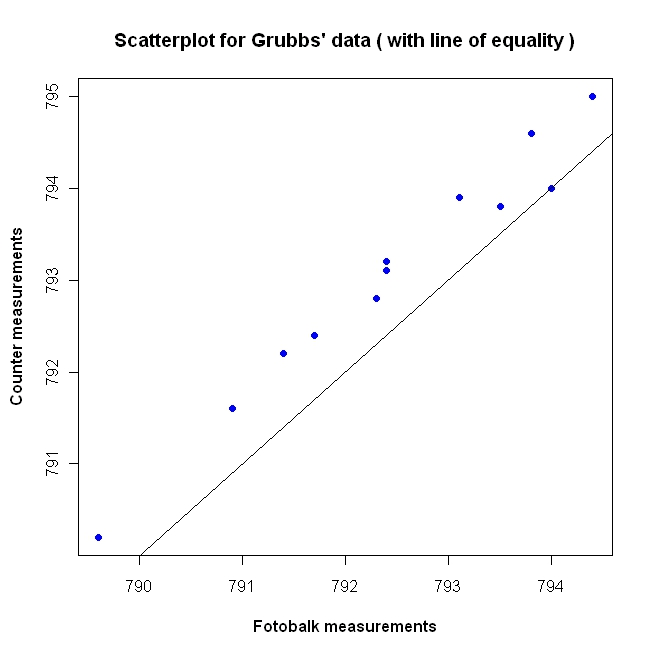
\includegraphics[width=130mm]{images/GrubbsScatter.jpeg}
			\caption{Scatter plot For Fotobalk and Counter Methods.}\label{GrubbsScatter}
		\end{center}
	\end{figure}
	
	In light of shortcomings associated with scatterplots,
	\citet*{BA83} recommend a further analysis of the data. Firstly
	case-wise differences of measurements of two methods $d_{i} =
	y_{1i}-y_{2i} \mbox{ for }i=1,2,..n$ on the same subject should be
	calculated, and then the average of those measurements ($a_{i} =
	(y_{1i} + y_{2i})/2 \mbox{ for }i=1,2,..n$). These differences and
	averages are then plotted. This methodology, now commonly known as
	the `Bland-Altman Plot', has proved very successful.
	\citet*{BA86}, which further develops the methodology, was found
	to be the sixth most cited paper of all time by the
	\citet{BAcite}. \cite{Dewitte} also commented on the rate at which
	prevalence of the Bland-Altman plot has developed in scientific
	literature. The Bland-Altman Plot has since become expected, and
	often obligatory, approach for presenting method comparison
	studies in many scientific journals \citep{hollis}. Furthermore
	\citet{BritHypSoc} recommend its use in papers pertaining to
	method comparison studies for the journal of the British
	Hypertension Society.
	
	The magnitude of the inter-method bias between the two methods is
	simply the average of the differences $\bar{d}$. The variances
	around this bias is estimated by the standard deviation of the
	differences $S(d)$. This inter-method bias is represented with a
	line on the Bland-Altman plot. These estimates are only meaningful
	if there is uniform inter-bias and variability throughout the
	range of measurements, which can be checked by visual inspection
	of the plot. In the case of Grubbs data the inter-method bias is
	$-0.61$ metres per second, and is indicated by the dashed line on
	Figure 1.2. By inspection of the plot, it is also possible to
	compare the precision of each method. Noticeably the differences
	tend to increase as the averages increase.
	
	
	\begin{table}[h!]
		\renewcommand\arraystretch{0.7}%
		\begin{center}
			\begin{tabular}{|c||c|c||c|c|}
				\hline
				Round & Fotobalk  & Counter  & Differences  & Averages  \\
				&  [F] & [C] & [F-C] &  [(F+C)/2] \\
				\hline
				1 & 793.8 & 794.6 & -0.8 & 794.2 \\
				2 & 793.1 & 793.9 & -0.8 & 793.5 \\
				3 & 792.4 & 793.2 & -0.8 & 792.8 \\
				4 & 794.0 & 794.0 & 0.0 & 794.0 \\
				5 & 791.4 & 792.2 & -0.8 & 791.8 \\
				6 & 792.4 & 793.1 & -0.7 & 792.8 \\
				7 & 791.7 & 792.4 & -0.7 & 792.0 \\
				8 & 792.3 & 792.8 & -0.5 & 792.5 \\
				9 & 789.6 & 790.2 & -0.6 & 789.9 \\
				10 & 794.4 & 795.0 & -0.6 & 794.7 \\
				11 & 790.9 & 791.6 & -0.7 & 791.2 \\
				12 & 793.5 & 793.8 & -0.3 & 793.6 \\
				\hline
			\end{tabular}
			\caption{Fotobalk and Counter methods: differences and averages.}
		\end{center}
	\end{table}
	
	\begin{table}[h!]
		\renewcommand\arraystretch{0.7}%
		\begin{center}
			\begin{tabular}{|c||c|c||c|c|}
				\hline
				Round & Fotobalk  & Terma  & Differences  & Averages  \\
				&  [F] & [T] & [F-T] &  [(F+T)/2] \\
				\hline
				1 & 793.80 & 793.20 & 0.60 & 793.50 \\
				2 & 793.10 & 793.30 & -0.20 & 793.20 \\
				3 & 792.40 & 792.60 & -0.20 & 792.50 \\
				4 & 794.00 & 793.80 & 0.20 & 793.90 \\
				5 & 791.40 & 791.60 & -0.20 & 791.50 \\
				6 & 792.40 & 791.60 & 0.80 & 792.00 \\
				7 & 791.70 & 791.60 & 0.10 & 791.65 \\
				8 & 792.30 & 792.40 & -0.10 & 792.35 \\
				9 & 789.60 & 788.50 & 1.10 & 789.05 \\
				10 & 794.40 & 794.70 & -0.30 & 794.55 \\
				11 & 790.90 & 791.30 & -0.40 & 791.10 \\
				12 & 793.50 & 793.50 & 0.00 & 793.50 \\
				
				\hline
			\end{tabular}
			\caption{Fotobalk and Terma methods: differences and averages.}
		\end{center}
	\end{table}
	
	\newpage
	
	


\subsection{Introduction to Limits of Agreement}
\begin{itemize}
	\item Comparing two methods of measurement is normally done by computing limits of agreement (LoA), i.e. prediction limits for
	a future difference between measurements with the two methods. When the difference is not constant it is not clear what
	this means, since the difference between the methods depends on the average; hence, unlike the case where the difference is
	constant, LoA cannot directly be translated into a prediction interval for a measurement by one method given that of another.
	\item The main point in the paper by Bland and Altman [1] is however different from the outlook in this paper; Bland and Altman
	mainly discuss whether two methods of measurement can be used interchangeably and how to assess this with the help of
	proper statistical methods to derive LoA, i.e. prediction limits for differences between two methods.
	This paper takes as starting point that the classical LoA can be converted to a prediction interval for one method given a
	measurement by the other (details in the next section). This sort of relationship can be shown in a plot as a line with slope 1
	and prediction limits as lines also with slope 1; applicable for the prediction both from method 1 to method 2 and vice versa. In
	the case of non-constant difference it would be desirable to be able to produce a similar plot, usable both ways. Thus, the aim
	of this paper is to produce a conversion from one method to another that also applies in the case where the difference between
	methods is not constant.
	\item In this paper, I set up a proper model for data for method comparison studies which in the case of constant difference between
	methods leads to the classical LoA, and in the case of linear bias gives a simple formula for the prediction. The paper only
	addresses the situation where only one measurement by each method is available, although replicate measurements by each
	method are desirable whenever possible [2]. Moreover, the situation with non-constant variance over the range of measurements
	is not covered either.
\end{itemize}
\newpage
\subsection{Discussion}
%----------------------------------------------------------------------------------------------------------------%
I have here proposed a simple twist to the results from regression of the differences on the sums in the case of a linear relationship
between two methods of measurement. It is consistent with the obvious underlying model, and exploits the fact that although
the parameters of the model cannot be estimated, those functions of the parameters that are needed for creating predictions
can be estimated.
%----------------------------------------------------------------------------------------------------------------%
The prediction limits provided have the attractive property that if the prediction line with limits is drawn in a coordinate
system, the chart will apply in both ways; hence, both the line and the limits are symmetric. Precisely as the prediction intervals
derived from the classical LoA are in the case where the difference between methods is constant.
%----------------------------------------------------------------------------------------------------------------%
The drawback is that the regression of the differences on the means ignores that the averages are correlated with the residuals
(i.e. the error terms), and therefore gives biased estimates if the slope linking the two methods is far from 1 or the residual
variances are very different. However, both of these are rather uncommon in method comparison studies, so the method proposed
here is widely applicable.
%----------------------------------------------------------------------------------------------------------------%
When considering LoA, the only feasible transformation is the log-transform, which gives LoA for the ratio of measurements,
which is immediately understandable. If, for example, the measurements are fractions where some are close to either 0 or 1 a
logit transform may be adequate. 

LoA would then be for (log) odds-ratios, not very easily understood. For other more arbitrarily
chosen transformation the situation may be even worse. But if a plot with conversion lines and limits are constructed, then the
plot is readily back-transformed to the original scale for practical use.
%---------------------------------------------------------------------------------

\subsection{Distribution of Maxima} It is possible to use Order
Statistics theory to assess conditional probabilities. With two
random variables $T_{0}$ and $T_{1}$, we define two variables $Z$
and $W$ such that they take the maximum and minimum values of the
pair of $T$ values.\subsection{Plot of the Maxima against the
	Minima}


In Figure 1,  The Maximas are plotted against their corresponding
minima. The Critical values of the Maxima and Minima are displayed
in the dotted lines.The Line of Equality depicts the obvious
logical constraint of the each Maximum value being greater than
its corresponding minimum value.



The scientific question at hand is the correct approach to
assessing whether two methods can be used interchangeably.
\citet{BA99} expresses this as follows:
\begin{quote}We want to
	know by how much (one) method is likely to differ from the
	(other), so that if it not enough to cause problems in the
	mathematical interpretation we can ... use the two
	interchangeably.
\end{quote}



Consequently, of the categories of method comparison study,
comparison studies, the second category, is of particular
importance, and the following discussion shall concentrate upon
it. Less emphasis shall be place on the other three categories.

\bigskip Further to \citet{BA86}, 'equivalence' of two methods expresses
that both can be used interchangeably.
\citet[p.49]{DunnSEME} remarks that this is a very restrictive
interpretation of equivalence, and that while agreement indicated
equivalence, equivalence does not necessarily reflect agreement.

The main difference between Myers proposed method and the Bland
Altman is that the random effects model is used to estimate the
within-subject variance after adjusting for known and unknown
variables. The Bland Altman approach uses one way analysis of
variance to estimate the within subject variance. In general, the
random effects model is an extension of the analysis of the ANOVA
method and it can adjust for many more covariates than the ANOVA
method






\newpage
\section{Conclusions about Existing Methodologies}

Scatterplots are recommended by \citet{BA83} for an initial
examination of the data, facilitating an initial judgement and
helping to identify potential outliers. They are not useful for a
thorough examination of the data. \citet{BritHypSoc} notes that
data points will tend to cluster around the line of equality,
obscuring interpretation.


The Bland Altman methodology is well noted for its ease of use,
and can be easily implemented with most software packages. Also it
doesn't require the practitioner to have more than basic
statistical training. The plot is quite informative about the
variability of the differences over the range of measurements. For
example, an inspection of the plot will indicate the 'fan effect'.
They also can be used to detect the presence of an outlier.

\citet{ludbrook97,ludbrook02}criticizes these plots on the
basis that they presents no information on effect of constant bias
or proportional bias. These plots are only practicable when both
methods measure in the same units. Hence they are totally
unsuitable for conversion problems. The limits of agreement are
somewhat arbitrarily constructed. They may or may not be suitable
for the data in question. It has been found that the limits given
are too wide to be acceptable. There is no guidance on how to deal
with outliers. Bland and Altman recognize effect they would have
on the limits of agreeement, but offer no guidance on how to
correct for those effects.

There is no formal testing procedure provided. Rather, it is upon
the practitioner opinion to judge the outcome of the methodology.










\section{Treatment of Outliers}
Bland and Altman attend to the issue of outliers in their 1986
paper, wherein they present a data set with an extreme outlier

\section{Bland Altman Plots In Literature}
\citet{mantha} contains a study the use of Bland Altman plots of
44 articles in several named journals over a two year period. 42
articles used Bland Altman's limits of agreement, wit the other
two used correlation and regression analyses. \citet{mantha}
remarks that 3 papers, from 42 mention predefined maximum width
for limits of agreement which would not impair medical care.

The conclusion of \citet{mantha} is that there are several
inadequacies and inconsistencies in the reporting of results ,and
that more standardization in the use of Bland Altman plots is
required. The authors recommend the prior determination of limits
of agreement before the study is carried out. This contention is
endorsed by \citet{lin}, which makes a similar recommendation for
the sample size, noting that\emph{sample sizes required either was
	not mentioned or no rationale for its choice was given}.

\begin{quote}
	In order to avoid the appearance of "data dredging", both the
	sample size and the (limits of agreement) should be specified and
	justified before the actual conduct of the trial. \citep{lin}
\end{quote}

\citet{Dewitte} remarks that the limits of agreement should be
compared to a clinically acceptable difference in measurements.
%%%%%%%%%%%%%%%%%%%%%%%%%%%%%%%%%%%%%%%%%%%%%%%%%%%%%%%%%%%%%%%%%%%%%%%%%
%4 Inappropriate assessment of Agreement       %%%%%%%%%%%%%%%%%%%%%%%%%%
%%%%%%%%%%%%%%%%%%%%%%%%%%%%%%%%%%%%%%%%%%%%%%%%%%%%%%%%%%%%%%%%%%%%%%%%%


\subsection{Gold Standard} This is considered to be the most
accurate measurement of a particular parameter.

\bibliographystyle{chicago}
\bibliography{DB-txfrbib}




\end{document} 

